\section{Independence, Dependence, and Circuits}\label{section_1.1}

\begin{definition}
  A \textit{matroid} is a set $E$, called the \textit{ground set},
  togehter with a collection $\Is$ of subsets of $E$, called
  \textit{independent sets} such that the following hold:
  \begin{enumerate}
    \item[($\Is1$)] $\0 \in \Is$.

    \item[($\Is2$)] If $I \in \Is$ and $J \subseteq I$, then $J \in
      \Is$.

    \item[($\Is3$)] If $I_1,I_2 \in \Is$, and $|I_1|<|I_2|$, then there
      exists an $e \in \com{I_2}{I_1}$ for which $I_1 \cup \{e\} \in \Is$.
  \end{enumerate}
  We call axiom ($\Is3$) the \textit{augmentation axiom}. We also
  write $I \cup e$ instead of $I \cup \{e\}$, when dealing with
  singletons. We denote a matroid by $\Mc=(E,\Is)$.
\end{definition}

\begin{definition}
  Let $\Mc=(E,\Is)$ a matroid. We call any set that is not in $\Is$ a
  \textit{dependent set} of $\Mc$.
\end{definition}

\begin{proposition}\label{proposition_1.1.1}
  Let $E$ be the set of column labels of an  $m \times n$ matrix $A$
  over a field $k$. Define $\Is$ the be the collection of all $I
  \subseteq E$ for which multisets of columns labeled by $I$ are sets,
  and are linearly independent in the vector space $V(m,k)$. Then
  $\Mc=(E,\Is)$ is a matroid.
\end{proposition}
\begin{proof}
  Since the columns labeled by the empty-set are linearly independent,
  we have $\0 \in \Is$. Now let $I \in \Is$ so the columns labeled by
  $I$ are linearly independent, and let $J \subseteq I$. Since the
  columns labeled by $I$ are linearly independent, the columns labeled
  by $J$ must also be linearly independent, so $J \in \Is$.

  Now, let $I_1, I_2 \in \Is$, with $|I_1|<|I_2|$. Let $W$ be the
  subspace spanned by the columns labeled by $I_1 \cup I_2$. Then
  $\dim{W} \geq |I_2|$. Now suppose for every $e \in \com{I_2}{I_1}$
  that $I_1 \cup e$ labels a set of linearly dependent columns. Then
  $W$ is contained in the span of the columns labeled by $I_1$ so that
  \begin{equation*}
    |I_2| \leq \dim{W} \leq |I_1|
  \end{equation*}
  but $|I_1|<|I_2|$, a contradiction. Therefore there must be at least
  one $e \in \com{I_2}{I_1}$ for which $I \cup e$ labels a set of
  linearly independent columns, hence $I \cup e \in \Is$. This makes
  $\Mc$ a matroid.
\end{proof}
\begin{corollary}
  Let $A$ be an $m \times n$ matrix over a field $k$, and let $E$ be
  the set of columns of $A$. Define $\Is$ the collection of all
  linearly independent sets of columns of $A$. Then $\Mc=(E,\Is)$
  defines a matroid on $A$.
\end{corollary}
\begin{proof}
  This is just an equivalent statement.
\end{proof}
\begin{corollary}
  Let $V$ be an $m$-dimensional vector space over a field $k$, and
  define $\Is$ the collection of all linearly independent sets of
  vectors of $V$. Then $\Mc=(V,\Is)$ defines a matroid on $V$.
\end{corollary}

\begin{definition}
  Let $A$ be an $m \times n$ matrix over a field $k$. We call the
  matroid $M$ obtained from $A$ by taking $\Is$ the set of all
  linearly independent combinations of columns of $A$ a
  \textit{vector matroid} and denote it $M[A]$. Similarly if $V$
  is an $m$-dimensional vector space on a field $k$, and $\Is$ is the
  collection of all linearly independent sets of vectors of $V$, then
  we denote the matroid obtained from $V$ by $M[V]$.
\end{definition}

\begin{example}\label{exampl_1.1}
  \begin{itemize}
    \item[(1)] The empty-set $\0$ together with $\Is=2^\0$ forms a
      matroid called the \textit{empty matroid}. Similarly, for any
      set $E$, and taking $\Is=2^E$, we call the resulting matroid
      $\Mc=(E,2^E)$ the \textit{trivial matroid}. These are the two
      most basic examples of matroids, since one matroid encompasses
      only the empty-set, and the other encompasses every subset of
      the ground set.

    \item[(2)] Consider the following $2 \times 5$ matrix over $\R$:
      \begin{equation*}
        A=
        \begin{pmatrix}
          1 & 0 & 0 & 1 & 1 \\
          0 & 1 & 0 & 0 & 1 \\
        \end{pmatrix}
      \end{equation*}
      and label the columns from left to right: $E=\{1, 2, 3, 4, 5\}$.
      Let $\Is$ be as defined in proposition \ref{proposition_1.1.1}.
      Then $\Is$ consists of the following subsets:
      \begin{center}
        \begin{tabular}{c c c c c }
          $\0$  & $\{1\}$ & $\{2\}$ & $\{4\}$ & $\{5\}$ \\
          $\{1, 2\}$  & $\{1, 5\}$  & $\{2, 4\}$  & $\{2, 5\}$ & $\{4, 5\}$  \\
        \end{tabular}
      \end{center}
      The dependent sets of $M[A]$ are:
      \begin{center}
        \begin{tabular}{c c c}
          $\{3\}$ & $\{1,3\}$ & $\{1,4\}$ \\
          $\{2,3\}$ & $\{3,4\}$ & $\{3,5\}$
        \end{tabular}
      \end{center}
      together with those sets of labels $X$ for which $|X|>3$.
      Indeed, the minimally dependent sets of $M[A]$ are:
      \begin{center}
        \begin{tabular}{c c c c}
          $\{3\}$ & $\{1,4\}$ & $\{1, 2, 5\}$ & $\{2,4,5\}$  \\
        \end{tabular}
      \end{center}
  \end{itemize}
\end{example}

\begin{definition}
  We call a minimally dependent set of a matroid a \textit{circuit}. A
  circuit having $n$ elements is called an \textit{$n$-circuit}.
\end{definition}

\begin{proposition}\label{proposition_1.1.2}
  If $\Cs$ is the collection of circuits of a matroid, then the
  following properties hold:
  \begin{enumerate}
    \item[($\Cs1$)] $\0 \notin \Cs$.

    \item[($\Cs2$)] If $C_1, C_2 \in \Cs$ and $C_1 \subseteq C_2$,
      then $C_1=C_2$.
  \end{enumerate}
\end{proposition}
\begin{proof}
  $(\Cs1)$ is a negation of $(\Is1)$, and $(\Cs2)$ follows from the
  definition of a circuit.
\end{proof}

\begin{proposition}[The Weak Circuit Elimination Axiom]\label{proposition_1.1.3}
  If $\Cc$ is the collection of circuits of a matroid, then the
  following property holds:
  \begin{enumerate}
    \item[($\Cs3$)] If $C_1,C_2 \in \Cs$ are distinct circuits, and $e
      \in C_1 \cap C_2$, then there exists a circuit $C \in \Cs$ such
      that
      \begin{equation*}
        C \subseteq \com{(C_1 \cup C_2)}{e}
      \end{equation*}
  \end{enumerate}
\end{proposition}
\begin{proof}
  Pick circuits $C_1,C_2 \in \Cs$ for which $(\Cs3)$ fails, that is,
  $\com{(C_1 \cup C_2)}{e}$ does not contain a circuit for some $e \in
  C_1 \cap C_2$. Then by the minimality of circuits, $\com{(C_1 \cup
  C_2)}{e} \in \Is$. Now, since $C_1 \neq C_2$ then $\com{C_2}{C_1}$
  is non-empty. Take an $f \in \com{C_2}{C_1}$. Then by minimality
  $\com{C_2}{f} \in \Is$.

  Now, choose a maximally independent $I \subseteq C_1 \cup C_2$ such
  that $\com{C_2}{f} \subseteq I$. Then $f \notin I$, and since $C_1$
  is a circuit, it contains some element $g \notin I$. Moreover since
  $f \in \com{C_2}{C_1}$, $f \neq g$. Hence we have:
  \begin{equation*}
    |I| \leq |\com{(C_1 \cup C_2)}{\{f,g\}}|=|C_1 \cup C_2|-2<|\com{(C_1 \cup C_2)}{e}|
  \end{equation*}
  Now, take $I_1=I$ and $I_2=\com{(C_1 \cup C_2)}{e}$. Then by the
  augmentation axiom, there exists an $h \in \com{I_2}{I_1}$ for which
  $I_1 \cup h \in \Is$. But this contradicts the maximality of
  $I_1=I$. Therefore $\com{(C_1 \cup C_2)}{e}$ must contain a circuit.
\end{proof}

\begin{theorem}\label{theorem_1.1.4}
  Let $E$ be a set and $\Cs$ a collection of subsets of $E$ satisfying
   $(\Cs1)$--$(\Cs3)$. Let $\Is$ be the collection of subsets of $E$
   which do not contain any member of $\Cs$. Then $\Is$ is the
   collection of independent sets of a matroid $\Mc$ on $E$.
\end{theorem}
\begin{proof}
  By $(\Cs1)$, $\0 \notin \Cs$, so $\0 \in \Cs$ by definition. Nowm
  let $I \in \Is$, and take $J \subseteq I$. Since $I$ contains no
  member of $\Cs$, then neither does $J$, hence  $J \in \Is$. So both
  $(\Is1)$ and $(\Is2)$ hold.

  Now, let $I_1, I_2 \in \Is$ with $|I_1|<|I_2|$, and suppose that
  $(\Is3)$ fails for $I_1$ and $I_2$. Now, $\Is$ contains a member
  which is a subset of $I_1 \cup I_2$, containing more elements than
  $I_1$. Choose such a set $I_3 \subseteq I_1 \cup I_2$ for which
  $|\com{I_1}{I_3}|$ is minimal. Now $\com{I_1}{I_3}$ is non-empty, so
  choose an element $e \in \com{I_1}{I_3}$. Then for any $f \in
  \com{I_3}{I_1}$, let $T_f=\com{(I_3 \cup e)}{f}$, then $T_f
  \subseteq I_1 \cup I_2$ and
  \begin{equation*}
    |\com{I_1}{T_f}|<|\com{I_1}{I_3}|
  \end{equation*}
  so by minimality, $T_f \notin \Is$. Therefore $T_f$ contains a
  member $C_f$ of $\Cs$. Then by definition $C_f \subseteq \com{(I_3
  \cup e)}{f}$, so that $f \notin C_f$, and $e \in C_f$. Otherwise
  $C_f \subseteq I_3$ which contradicts the independence of $I_3$.

  Now let $g \in \com{I_3}{I_1}$. Observe that if $C_g \cap
  (\com{I_3}{I_1})=\0$, then $C_g \subseteq \com{((I_1 \cap I_3) \cup
  e)}{g} \subseteq I_1$, which contradicts the independence of $I_1$.
  Then $C_g \cap (\com{I_3}{I_1}) \neq \0$, so there exists an
  element $h \in C_g \cap (\com{I_3}{I_1})$, with $C_h \neq C_g$,
  since $h \notin C_g$. Now, we have that $e \in C_g \cap C_h$, so by
  $(\Cs3)$, there exists an element $C \in \Cs$ such that
  \begin{equation*}
    C \subseteq \com{(C_g \cup C_h)}{e}
  \end{equation*}
  But $C_g,C_h \subseteq I_3 \cup e$, so that $C \subseteq I_3$, which
  contradicts the independence of $I_3$. It must follow then that
  $(\Is3)$ holds, and $\Is$ is the collection of independent sets of a
  matroid $\Mc=(E,\Is)$.
\end{proof}
\begin{corollary}
  $\Cs$ is the collection of circuits of the matroid $\Mc$.
\end{corollary}
\begin{proof}
  We observe from definition, and the axioms $(\Cs1)$--$(\Cs3)$, that
  the following statements are equivalent:
  \begin{enumerate}
    \item[(1)] $C$ is a circuit.

    \item [(2)] $C \notin \Is$, and $\com{C}{x} \in \Is$ for every $x
      \in C$.

    \item[(3)] $\Cs$ has a member $C'$ which is a subset of $C$, but
      not a proper subset of $C$.

    \item[(4)] $C \in \Cs$.
  \end{enumerate}
\end{proof}

Now, we have shown the equivalence between two axioms for what a
matroid is. The first set of axioms, $(\Is):(\Is1)$--$(\Is3)$ cover the
independence axioms. That is, they define what the independent sets of
a matroid are. The second set $(\Cs):(\Cs1)$--$(\Cs3)$ define what the
circuits of an axiom are. We show a digraph of the equivalence of the
axioms below:
\begin{figure}[h]
  \centering
  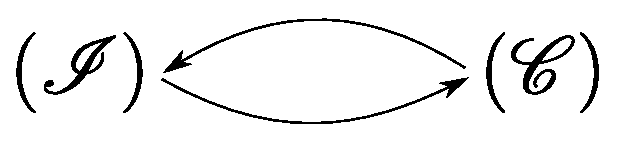
\includegraphics[scale=0.5]{figures/Chapter1/equiv_def_1.eps}
  \caption{There is an equivalence between the axioms $(\Is)$ defining
  indpendent sets with the axioms $(\Cs)$ defining circuits.}
  \label{figure_1.1}
\end{figure}
